\documentclass{tufte-handout}

%\geometry{showframe}% for debugging purposes -- displays the margins

\usepackage[spanish, es-tabla]{babel}
\usepackage{amsmath}
\newtheorem{theorem}{Postulado}

% Set up the images/graphics package
\usepackage{graphicx}
\setkeys{Gin}{width=\linewidth,totalheight=\textheight,keepaspectratio}
\graphicspath{{figs/}{figs/retratos/}{graphics/}}

\title[Química Física II: Tema 2, Postulados]{
Tema 2: Postulados de la Mecánica Cuántica}
%\author{David De Sancho}
\date{}  % if the \date{} command is left out, the current date will be used

% The following package makes prettier tables.  We're all about the bling!
\usepackage{booktabs}

% The units package provides nice, non-stacked fractions and better spacing
% for units.
\usepackage{units}

% The fancyvrb package lets us customize the formatting of verbatim
% environments.  We use a slightly smaller font.
\usepackage{fancyvrb}
\fvset{fontsize=\normalsize}

% Small sections of multiple columns
\usepackage{multicol}

% Provides paragraphs of dummy text
\usepackage{lipsum}

% These commands are used to pretty-print LaTeX commands
\newcommand{\doccmd}[1]{\texttt{\textbackslash#1}}% command name -- adds backslash automatically
\newcommand{\docopt}[1]{\ensuremath{\langle}\textrm{\textit{#1}}\ensuremath{\rangle}}% optional command argument
\newcommand{\docarg}[1]{\textrm{\textit{#1}}}% (required) command argument
\newenvironment{docspec}{\begin{quote}\noindent}{\end{quote}}% command specification environment
\newcommand{\docenv}[1]{\textsf{#1}}% environment name
\newcommand{\docpkg}[1]{\texttt{#1}}% package name
\newcommand{\doccls}[1]{\texttt{#1}}% document class name
\newcommand{\docclsopt}[1]{\texttt{#1}}% document class option name

% Retratos históricos en el margen. Todas las imágenes son de dominio
% público y proceden de Wikimedia Commons; la procedencia completa está en
% figs/retratos/CREDITOS.md.
%
% Es un marginfigure SIN \caption: así no consume números de figura y no
% desplaza los \ref existentes. El % tras el corchete no es opcional (sin él
% la imagen se sale del margen). El razonamiento completo está comentado en
% el preámbulo de tema01.tex.
\makeatletter
\setlength{\@fptop}{0pt}
\makeatother

\newcommand{\retrato}[2]{%
  \begin{marginfigure}[\baselineskip]%
    \includegraphics[width=\linewidth]{#1}\par
    \vspace{0.4ex}{\footnotesize #2}\par
    \vspace*{\baselineskip}
  \end{marginfigure}}

\begin{document}

\maketitle% this prints the handout title, author, and date

\begin{abstract}
\noindent La Mecánica Cuántica está basada en una serie de
postulados.\sidenote{Los postulados son, según el diccionario
de la Real Academia de la Lengua, ``proposiciones cuya
verdad se admite sin pruebas y que sirven de base para
ulteriores razonamientos''.} Un formalismo construido sobre
postulados se justifica por sus consecuencias: comparando con
el experimento los resultados a los que conduce.
A continuación introduciremos
los postulados de la Mecánica Cuántica, que usaremos 
como fundamento para describir más adelante sistemas
sencillos.
\end{abstract}

%\printclassoptions



\section{Estados y funciones de onda}
En el caso de la Mecánica Clásica, el estado de una partícula
viene determinado por las  coordenadas de posición ($x, y, z$) 
y momento ($p_x, p_y, p_z$). Así, su evolución temporal viene
dada por las ecuaciones de Newton, que definen de manera 
determinista su trayectoria. En Mecánica Cuántica esa
descripción determinista no es posible, y el papel de la
trayectoria lo pasa a desempeñar otro objeto. Esto nos lleva
al primero de nuestros postulados:

\begin{theorem}
Todas las propiedades observables de un sistema físico 
están contenidas en su función de onda, $\Psi(q,t)$,
dependiente de las coordenadas ($q$) de las
partículas que componen el sistema y del tiempo ($t$). 
\end{theorem}

En Mecánica Cuántica, por tanto, el concepto de 
trayectoria es reemplazado por la \textbf{función de
onda}, que contiene toda la información dinámica 
sobre el sistema.

\section{Interpretación de la función de onda}
\retrato{retrato_born_v1.jpg}{Max Born (1882--1970), que en 1926 dio a
$|\psi|^2$ su significado probabilístico.}%
Para desarrollar una intuición sobre el significado
de la función de onda es útil recurrir a la 
denominada \textbf{interpretación de 
Born}, que también enunciamos en la forma de 
postulado.
\begin{theorem} 
La probabilidad de que una partícula se encuentre en un
elemento de volumen $d\tau$ alrededor del punto $r$ es
proporcional a $|\psi(r)|^2d\tau=\psi^\star\psi\,d\tau$
\end{theorem}
El cuadrado de la función de onda es por tanto una
\textbf{densidad de probabilidad} (Figura~\ref{fig:psi-psi2}).
Integrando esa densidad
sobre una región finita del espacio obtenemos la probabilidad
de encontrar la partícula en ella. Puesto que la suma de
todas las probabilidades debe ser igual a la unidad, la
función de onda debe cumplir una condición de
normalización,
\begin{equation}
    N^2\int_{-\infty}^\infty\psi^\star\psi\,dx=1
    \label{eq:norm}
\end{equation}
donde $N$ es la \textbf{constante de normalización}, que no
es un parámetro libre: queda determinada sin más que
despejarla de la Ecuación~\ref{eq:norm},
\begin{equation}
    N=\left(\int_{-\infty}^\infty\psi^\star\psi\,dx\right)^{-1/2}
    \label{eq:cte-norm}
\end{equation}
De aquí en adelante daremos por supuesto que la función de
onda ya está normalizada; es decir, escribiremos $\psi$
donde en rigor deberíamos escribir $N\psi$.

\begin{figure}
  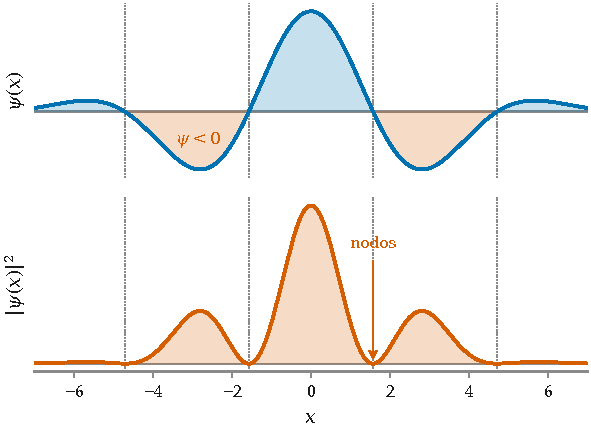
\includegraphics{postulados_psi-psi2_v1.pdf}
  \caption{Arriba, una función de onda normalizada $\psi(x)$, que toma
  valores tanto positivos como negativos. Abajo, la densidad de probabilidad
  $|\psi(x)|^2$ que se deriva de ella. Al elevar al cuadrado ocurren dos cosas:
  la densidad es positiva en todo punto ---una probabilidad negativa no
  significaría nada--- y se anula exactamente donde $\psi$ cambia de signo.
  Esos puntos son los nodos, y en ellos la probabilidad de encontrar la
  partícula es cero.}
  \label{fig:psi-psi2}
\end{figure}

En ocasiones, para el caso tridimensional, puede 
ser más conveniente escribir esta condición de 
normalización en coordenadas esféricas, es decir,
en función del radio $r$, la colatitud $\theta$
y el ángulo azimutal $\phi$. La interconversión
entre coordenadas cartesianas y esféricas es 
trivial, 
\begin{equation}
  \begin{array}{@{}ll@{}}
    x = & r\sin\theta\cos\phi \\
    y = & r\sin\theta\sin\phi \\
    z = & r\cos\theta
  \end{array}
\end{equation}
de tal manera que la condición de normalización que 
expresábamos en una sola dimensión en la 
Ecuación~\ref{eq:norm} se puede reescribir usando
$d\tau=r^2\sin\theta\,dr\,d\theta\,d\phi$ y modificando
los límites de integración de la siguiente manera
\begin{equation}
    \int\psi^\star\psi\,d\tau=
    \int_0^\infty\!\!\int_0^\pi\!\!\int_0^{2\pi}
    \psi^\star\psi\,r^2\sin\theta\,dr\,d\theta\,d\phi=1
    \label{eq:norm-esfericas}
\end{equation}

La interpretación de Born y la ecuación de Schrödinger
que, como veremos más adelante, es una ecuación
diferencial de segundo orden, introducen una serie de
requisitos para las funciones de onda aceptables
(Figura~\ref{fig:admisibles}):
\begin{itemize}
    \item Debe ser unívoca, es decir, no debe 
    estar definida con más de un valor en cada punto.
    \item Debe tener un cuadrado integrable.
    \item Debe ser continua.
    \item Debe ser derivable.
\end{itemize}

\begin{figure}
  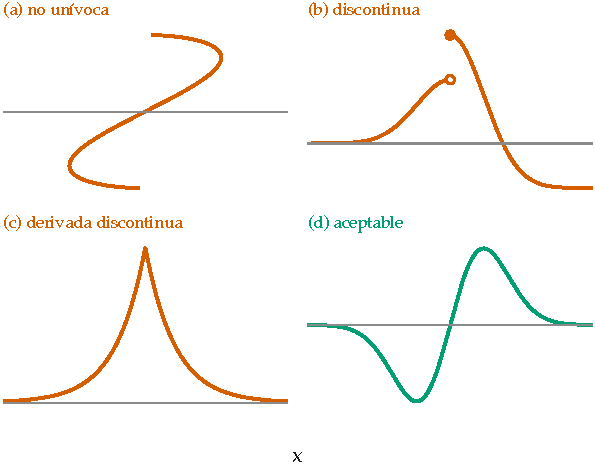
\includegraphics{postulados_funciones-admisibles_v1.pdf}
  \caption{Tres funciones que no pueden ser funciones de onda y una que sí.
  (a) toma más de un valor en cada punto; (b) presenta un salto, de modo que
  no es continua; (c) es continua pero su derivada no lo es, y la ecuación de
  Schrödinger contiene una derivada segunda; (d) cumple todos los requisitos.}
  \label{fig:admisibles}
\end{figure}


\section{Observables y operadores}
\begin{theorem}
Los observables se representan mediante operadores 
hermíticos.
\end{theorem}
Para entender este postulado debemos definir primero
los operadores. Un operador, $\hat{\Omega}$, no es sino una
regla que transforma una función de onda en otra:
\begin{equation}
    \psi(q,t)\xrightarrow{\hat{\Omega}}\psi'(q,t)
\end{equation}
Un ejemplo de operador es el operador
diferencial con respecto de $x$, $\hat{D}_x=\frac{d}{dx}$.
Al aplicarlo sobre la función \textit{seno}, obtenemos
la función \textit{coseno}.
\begin{equation}
    \hat{D}_x\sin x=\frac{d}{dx}\sin x =\cos x
\end{equation}
Un \textbf{operador lineal} es un tipo especial de operador
que satisface las siguientes relaciones
\begin{equation}
      \begin{array}{rl}
        \hat{\Omega}(\psi+\phi) &=\hat{\Omega}\psi + \hat{\Omega}\phi\\
        \hat{\Omega}c\psi &=c\hat{\Omega}\psi
    \end{array}
\end{equation}

De todas las formas en que un operador puede actuar sobre
una función, hay una que nos interesa especialmente en
Mecánica Cuántica: aquella en que el resultado es la misma
función multiplicada por un número. Cuando esto ocurre
decimos que tenemos una \textbf{ecuación de valores
propios}:
\begin{equation}
    \hat{\Omega}\Psi(q,t)=\omega\Psi(q,t)
\end{equation}
donde $\omega$ es el valor propio (\textit{eigenvalue})
correspondiente al operador $\hat{\Omega}$. Cuando
encontramos esta propiedad, entonces decimos que $\Psi$ 
es función propia (\textit{eigenfunction}) de este
operador. Este tipo de expresión es la que nos vamos a
encontrar en el caso del operador hamiltoniano, 
$\hat{H}$, para la energía total pero también para 
otros observables que mostramos en la 
Tabla~\ref{tab:operators}.

\begin{table}[h]
  \begin{center}
    %\footnotesize%
    \small
    \begin{tabular}{ll}
      \toprule
      Nombre & Expresión \\
      \midrule
      Posición & $\hat{x}=x$ \\
      Momento lineal & $\hat{p}_x=-i\hbar \frac{\partial}{\partial x}$ \\
      Energía cinética & $\hat{K}=\frac{\hat{p}_x^2}{2m}=
      -\frac{\hbar^2}{2m}\frac{\partial^2}{\partial x^2}$\\
      Energía potencial & $\hat{V}=V(x,y,z)$ \\
      Hamiltoniano & $\hat{H}=\hat{K}+\hat{V}$ \\
      \bottomrule
    \end{tabular}
  \end{center}
  \caption{Operadores habituales en Mecánica Cuántica.}
  \label{tab:operators}
\end{table}

Finalmente, un \textbf{operador hermítico} es el que
satisface la siguiente relación
\begin{equation}
    \int\psi_i^\star\hat{\Omega}\psi_j\,d\tau=
    \bigg\{\int\psi_j^\star\hat{\Omega}\psi_i\,d\tau\bigg\}^\star
\end{equation}
Estos operadores tienen dos propiedades especiales:
\begin{itemize}
    \item Sus valores propios son reales.
    \item Sus funciones propias correspondientes a valores
    propios \emph{distintos} son ortogonales, es decir, si
    $\omega_1\neq\omega_2$, entonces
    $\int\psi_1^\star\psi_2\,d\tau=0$.\sidenote{Cuando dos o
    más funciones propias comparten el mismo valor propio
    decimos que el nivel está \textbf{degenerado}. En ese caso
    no tienen por qué ser ortogonales entre sí, pero siempre
    se pueden sustituir por combinaciones lineales suyas que
    sí lo sean.}
\end{itemize}
El conjunto de funciones propias de un operador
hermítico forma un \textbf{conjunto completo}.

\section{El resultado de una medida}
\begin{theorem}
Toda medida individual de un observable $\Omega$ devuelve
uno de los valores propios $\omega_k$ del operador
$\hat{\Omega}$ asociado, y ningún otro valor.
\end{theorem}
Si la función de onda es función propia de $\hat{\Omega}$
el resultado está determinado, porque todas las medidas
devuelven el mismo valor propio. Cuando no lo es, en
cambio, no podemos predecir el resultado de una medida
concreta. Sí podemos, sin embargo, expresar la
función de onda como una combinación lineal o
\textbf{superposición} de un conjunto de funciones
propias
\begin{equation}
\psi =  c_1\psi_1 + c_2\psi_2 + \dots = \sum_kc_k\psi_k
\label{eq:superposicion}
\end{equation}
En esta expresión los coeficientes $c_k$ son números
complejos y las funciones $\psi_k$ corresponden a estados
distintos del sistema. Que cualquier función de onda admita
este desarrollo no es una suposición: es justamente lo que
significa que las $\psi_k$ formen un conjunto completo.

Cuando se realiza una medida se obtiene el valor propio
$\omega_k$ correspondiente a una de las funciones propias
$\psi_k$, con una probabilidad que viene dada por el
cuadrado del módulo de su coeficiente en la combinación
lineal,\sidenote{Que las probabilidades sumen la unidad,
$\sum_k|c_k|^2=1$, no es una condición adicional: es la
condición de normalización de la Ecuación~\ref{eq:norm}
escrita en la base de las $\psi_k$.}
\begin{equation}
    P(\omega_k)=|c_k|^2
    \label{eq:prob-ck}
\end{equation}
No podemos, por tanto, predecir el resultado de una medida
aislada, sino sólo la frecuencia con la que aparecerá cada
uno de los valores posibles. Lo que sí queda determinado es
el promedio sobre un gran número de medidas, el
\textbf{valor esperado} (\textit{expectation value}),
\begin{equation}
    \langle\Omega\rangle=\sum_k|c_k|^2\omega_k=
    \int\psi^\star\hat{\Omega}\psi\,d\tau
    \label{eq:valor-esperado}
\end{equation}



\section{La ecuación de Schrödinger}
\retrato{retrato_schrodinger_v1.jpg}{Erwin Schrödinger (1887--1961)
en 1933, el año en que compartió el Nobel con Dirac.}%
\begin{theorem}
La función de onda evoluciona en el tiempo de acuerdo 
con la ecuación de Schrödinger dependiente del tiempo:
\begin{equation}
    \hat{H}\Psi = i\hbar\frac{\partial \Psi}{\partial t}
\end{equation}
\end{theorem}
Como conocemos el operador hamiltoniano, $\hat{H}$ (ver
Tabla \ref{tab:operators}), podemos escribir si trabajamos
en una sola dimensión
\begin{equation}
    \hat{H}\Psi = 
      -\frac{\hbar^2}{2m}\frac{\partial^2}{\partial x^2}\Psi + V(x)\Psi = i\hbar\frac{\partial \Psi}{\partial t}
\end{equation}
En el caso de los estados estacionarios 
se puede separar la parte de la función de onda
que depende de las coordenadas de la parte que 
depende del tiempo,
\begin{equation}
    \Psi(q,t)=\psi(q)\tau(t)
\end{equation}
El hamiltoniano actúa sólo sobre la parte espacial, de modo
que
\begin{equation}
    \hat{H}\Psi(q,t)=
    \tau(t)\hat{H}\psi(q)=
    i\hbar\frac{\partial\psi(q)\tau(t)}{\partial t}=
    i\hbar\psi(q)\frac{\partial \tau(t)}{\partial t}
\end{equation}
Dividiendo ahora por $\psi(q)\tau(t)$ separamos por completo
las dos variables,
\begin{equation}
    \frac{1}{\psi(q)}\hat{H}\psi(q) = \frac{i\hbar}{\tau(t)}\frac{\partial \tau(t)}{\partial t}= E
    \label{eq:schro-2}
\end{equation}
El miembro de la izquierda depende sólo de las coordenadas
y el del centro sólo del tiempo, de modo que ambos han de
ser iguales a una misma constante, $E$, que identificamos
con la energía. La Ecuación~\ref{eq:schro-2} contiene por
tanto dos ecuaciones independientes. La primera de ellas es
la \textbf{ecuación de Schrödinger independiente del
tiempo},
\begin{equation}
    \hat{H}\psi(q)=E\psi(q)
    \label{eq:schro-independiente}
\end{equation}
que es una ecuación de valores propios del hamiltoniano y
es la que resolveremos en los temas
siguientes.\sidenote{Resolverla equivale a encontrar a la
vez las funciones propias $\psi(q)$, que son los estados
estacionarios accesibles al sistema, y sus valores propios
$E$, que son las energías permitidas.}
A partir de los dos términos a la derecha de la Ecuación
\ref{eq:schro-2} obtenemos la segunda, cuya solución es
\begin{equation}
    \tau(t)=A\exp(-iEt/\hbar)
    \label{eq:tau-t}
\end{equation}
Por tanto la función de onda para un estado estacionario
es
\begin{equation}
    \Psi(q,t)=\psi(q)\exp(-iEt/\hbar)
    \label{eq:estacionario}
\end{equation}
Si calculamos la densidad de probabilidad veremos por qué a
estos estados los llamamos \textbf{estacionarios}: al tomar
el módulo al cuadrado, las dos exponenciales se cancelan
\begin{equation}
    |\Psi(q,t)|^2=\Psi^\star\Psi=
    \psi^\star(q)e^{+iEt/\hbar}\,\psi(q)e^{-iEt/\hbar}=
    |\psi(q)|^2
    \label{eq:densidad-estacionaria}
\end{equation}
de modo que la densidad de probabilidad no depende del
tiempo, aunque la función de onda sí lo haga.
Estos estados tienen además una energía definida, $E$.
En un estado estacionario, todo observable cuyo operador
conmuta con el hamiltoniano tiene un valor bien definido y
constante en el tiempo. Son el equivalente cuántico de las
constantes de movimiento de la mecánica clásica.

\section{El principio de incertidumbre}
Con los operadores ya definidos podemos volver sobre el
\textbf{principio de incertidumbre} enunciado por
\textbf{Werner Heisenberg}. Como comentamos en el Tema 1,
el principio establece en su formulación más básica que no
se puede determinar simultáneamente y con precisión
arbitraria el momento y la posición de una partícula. 

Supongamos que queremos describir una partícula cada vez
mejor localizada en un punto del espacio. Utilizando el
principio de superposición, podemos construir esa
descripción combinando un número creciente de ondas 
armónicas, es decir, generando un paquete de
ondas (\textit{wave packet}). Cuantas más ondas sumamos,
más estrecho es el paquete y menor la incertidumbre en la
posición ($\Delta x\rightarrow 0$).
Pero a su vez las distintas contribuciones a la función 
de onda tienen valores del momento lineal cada vez más
dispares, lo que hace crecer sin límite la incertidumbre en
el momento ($\Delta p\rightarrow\infty$). Ninguno de los dos
extremos es alcanzable: son límites idealizados que
muestran que, si ganamos certeza en uno de los dos valores,
la perdemos en el otro (Figura~\ref{fig:paquete}).

\begin{figure*}
  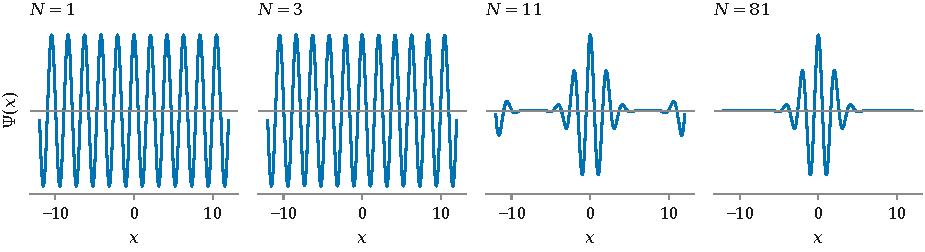
\includegraphics{incertidumbre_paquete-ondas_v1.pdf}
  \caption{Construcción de un paquete de ondas por superposición de $N$ ondas
  armónicas de distinto momento. Con una sola onda ($N=1$) el momento
  está perfectamente definido pero la partícula está deslocalizada por todo el
  eje. Al aumentar $N$ el paquete se estrecha ---la posición se determina cada
  vez mejor--- a costa de mezclar cada vez más valores del momento.}
  \label{fig:paquete}
\end{figure*}

El principio de incertidumbre, formulado típicamente para
$p$ y $q$, es en realidad más general. Si para cada 
operador $\hat{\Omega}$ definimos su incertidumbre
$\Delta\Omega$ como la desviación típica
\begin{equation}
    (\Delta\Omega)^2=\sigma^2_\Omega=\langle (\hat{\Omega} - \langle \Omega\rangle)^2 \rangle=
    \langle\hat{\Omega}^2\rangle - \langle\Omega\rangle^2
    \label{eq:varianza}
\end{equation}
queda claro que $\Delta x$ y $\Delta p$ no son errores del
aparato de medida, sino una propiedad del estado del sistema:
miden su dispersión intrínseca. Con esta definición, el
principio de incertidumbre relaciona las incertidumbres de dos
\textbf{variables complementarias} de tal modo que
\begin{equation}
\Delta\Omega_1\Delta\Omega_2\geq
\frac{1}{2}\left|\langle[\hat{\Omega}_1,\hat{\Omega}_2]\rangle\right|
\end{equation}
\begin{figure}[!htb]
  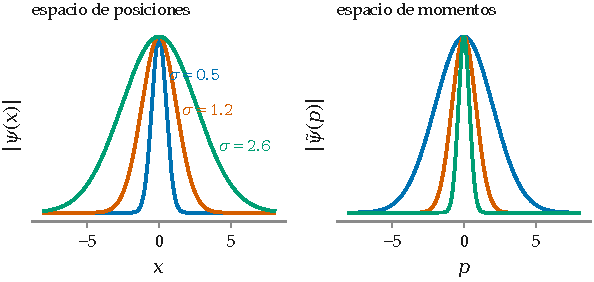
\includegraphics{incertidumbre_x-p_v1.pdf}
  \caption{La misma función de onda vista en el espacio de posiciones
  (izquierda) y en el de momentos (derecha), para tres anchuras $\sigma$. Las
  dos descripciones no son independientes: estrechar la primera ensancha
  necesariamente la segunda, de modo que el producto
  $\Delta x\,\Delta p$ nunca baja de $\hbar/2$.}
  \label{fig:x-p}
\end{figure}
donde  usamos el conmutador  $[\hat{\Omega}_1,\hat{\Omega}_2] =
\hat{\Omega}_1\hat{\Omega}_2 -\hat{\Omega}_2\hat{\Omega}_1$.
Son complementarias aquellas variables que no conmutan y para
las que se cumple 
$\hat{\Omega}_1(\hat{\Omega}_2\psi)\neq\hat{\Omega}_2(\hat{\Omega}_1\psi)$.
En el caso particular de la posición y el momento obtenemos que
\begin{equation}
    [\hat{x},\hat{p}_x] = i\hbar
\end{equation}
y por tanto son operadores
complementarios (Figura~\ref{fig:x-p}). Por el contrario, cuando
dos operadores hermíticos conmutan decimos 
que son \textbf{compatibles}, y comparten un conjunto
completo de funciones propias, $\psi_n$.

% La Figura 4 quedaba pendiente al llegar aquí y la clase sólo vacía los
% flotantes después de componer el título, con lo que el título se quedaba
% solo al pie de la página. La barrera explícita los coloca antes.
\FloatBarrier
\section{Principio de exclusión o de Pauli}
\retrato{retrato_pauli_v1.jpg}{Wolfgang Pauli (1900--1958).}%
Por último introduciremos una contribución decisiva
al desarrollo de la Mecánica Cuántica. Las partículas
cuánticas poseen una propiedad fundamental, el
\textit{spin} o espín, $s$, que toma un valor entero o
semientero característico de cada partícula y que fue
introducida por \textbf{Wolfgang Pauli} como lo que él
denominaba una bivalencia no describible clásicamente
(``classically non-describable two-valuedness'').\sidenote{No
debe confundirse con la dualidad onda-partícula del Tema 1:
aquí se trata de que una misma propiedad admita exactamente
dos valores.}

El espín permite clasificar las partículas en dos tipos.
Las de espín semientero, como los electrones, protones o
neutrones, se denominan \textbf{fermiones}; las de espín
entero, como los fotones, \textbf{bosones}. La distinción
es la que da contenido al último de nuestros postulados:
\begin{theorem}
La función de onda de un colectivo de partículas idénticas
debe ser simétrica (bosones) o antisimétrica (fermiones)
frente al intercambio de dos cualesquiera de ellas,
\begin{equation*}
    \Psi(q_1, \dots, q_i, \dots, q_j, \dots, q_N)=\pm 
    \Psi(q_1, \dots, q_j, \dots, q_i, \dots, q_N)
\end{equation*}
donde el signo $+$ corresponde a los bosones y el $-$ a los
fermiones.
\end{theorem}
La consecuencia de la antisimetría es que dos fermiones no
pueden ocupar simultáneamente el mismo estado de una
partícula, mientras que los bosones sí pueden coexistir en
un estado idéntico. Desarrollaremos esta idea, y sus
consecuencias sobre la estructura electrónica de los
átomos, en el Tema 7.

\end{document}
